% !TeX spellcheck = it_IT
% !TEX TS-program = pdflatex
% !TEX root = ../main.tex


% ********************************************************************
\section{Implementazione e prototipo}
\label{sec:prototipo}
% ********************************************************************


\subsection{Login e autenticazione}
L'autenticazione all'interno della piattaforma adotta il protocollo \gls{siwe} sostituendo il modello tradizionale basato sull’utilizzo di credenziali tradizionali quali \textit{username} e \textit{password}, coerentemente con il paradigma Web3. L’identità dell’utente è infatti associata in modo univoco al possesso di un \textit{wallet}. 

Il flusso di \textit{login} ha inizio con la connessione del \textit{wallet} dell’utente, a partire dal quale il \textit{front-end} ottiene l’indirizzo pubblico associato. Tale indirizzo viene inviato al \textit{back-end}, che a sua volta, genera un \textit{nonce}, ovvero un valore casuale e univoco utilizzato per prevenire attacchi di tipo \textit{replay}. 
Il \textit{nonce} viene associato temporaneamente all’utente, tramite sessione o persistenza nel database, e restituito al \textit{front-end}.

Successivamente, il \textit{front-end} costruisce un messaggio conforme allo standard \gls{siwe}, includendo il \textit{nonce} ricevuto, e richiede all’utente di firmarlo tramite il proprio \textit{wallet}. Il messaggio firmato e la relativa firma vengono quindi inviati al \textit{back-end}, che procede alla verifica dell’autenticazione. In particolare, il \textit{server} controlla sia che l’indirizzo estratto crittograficamente dalla firma coincida con quello dichiarato sia che il \textit{nonce} contenuto nel messaggio corrisponda a quello attualmente valido, impedendo il riutilizzo di firme precedenti.

Solo se entrambi i controlli vanno a buon fine, l’autenticazione viene considerata valida e viene avviata una sessione applicativa. In fase di primo accesso, l’utente viene registrato automaticamente nel sistema, mentre per accessi successivi vengono aggiornate le informazioni di sessione. Al termine del processo, il \textit{nonce} viene rigenerato e quello precedente invalidato, garantendo la sicurezza delle autenticazioni future.

Infine, il \textit{front-end} utilizza il \textit{cookie} di sessione per recuperare le informazioni dell’utente autenticato e completare il processo di accesso all’applicazione.



\begin{figure}[h]
	\centering
	\includegraphics[trim={0 0 0 1.8cm}, clip, width=1\textwidth]{images/sequenza_login.jpeg}
	\caption{Diagramma di sequenza del processo di \textit{login}.}
	\label{fig:login}
\end{figure}
\clearpage


\subsubsection{Ente}
L’Ente beneficiario rappresenta l’attore abilitato alla creazione delle iniziative di raccolta fondi sulla piattaforma. \\
Il suo riconoscimento avviene durante la fase di autenticazione, contestualmente alla verifica della firma crittografica dell’utente. \\
In particolare, durante la procedura di \textit{login}, il \textit{back-end} accerta l’identità dell’utente e interroga la blockchain per verificare se l’indirizzo del \textit{wallet} risulti associato a un NFT non trasferibile (\textit{Soulbound Token}) denominato \textit{ETS}.
Tale \textit{token} funge dunque da attestazione crittografica dello stato di ente autorizzato al'interno del sistema e viene rilasciato esclusivamente a seguito di un processo di registrazione e verifica \textit{off-chain}.\\
Una volta autenticato, il sistema abilita le funzionalità riservate a questa tipologia di utente, il quale può avviare nuove raccolte o contribuire ai progetti di altri enti, mentre gli è preclusa, per motivi di integrità del sistema, la possibilità di effettuare donazioni verso le proprie iniziative.


\subsection{Dashboard donatore}
La \textit{dashboard} del donatore è l'interfaccia attraverso la quale gli utenti possono interagire direttamente con la piattaforma a seguito della procedura di autenticazione. Essa è progettata per fornire una visione sintetica e intuitiva delle iniziative di \gls{cf} attive, permettendo all'utente di monitorarne lo stato di avanzamento attraverso indicatori chiave quali il \textit{budget} raccolto, il numero di donatori coinvolti e la data di scadenza. \\
Una volta selezionata l’iniziativa di interesse, l’utente ha la possibilità di procedere con l’operazione di donazione. In particolare, il sistema adotta il meccanismo di raccolta \textit{keep-it-all}, in base al quale l’Ente beneficiario conserva i fondi raccolti anche qualora l’obiettivo economico prefissato non venga raggiunto entro i termini prestabiliti.
Tale scelta progettuale risulta coerente con la categoria di Enti autorizzati alla creazione delle iniziative sulla piattaforma, individuati esclusivamente negli Enti del Terzo Settore, per i quali anche contributi parziali possono risultare funzionali al perseguimento delle finalità sociali.


% l'utente non può sovraeccedere il target, quindi non può effettuare donazioni che siano più grandi della quota da donare 
% se un utente paga tutto e raggiunge il target per coerenza non può donare altri soldi  può donare altri soldi 



\begin{figure}[h]
	\centering
	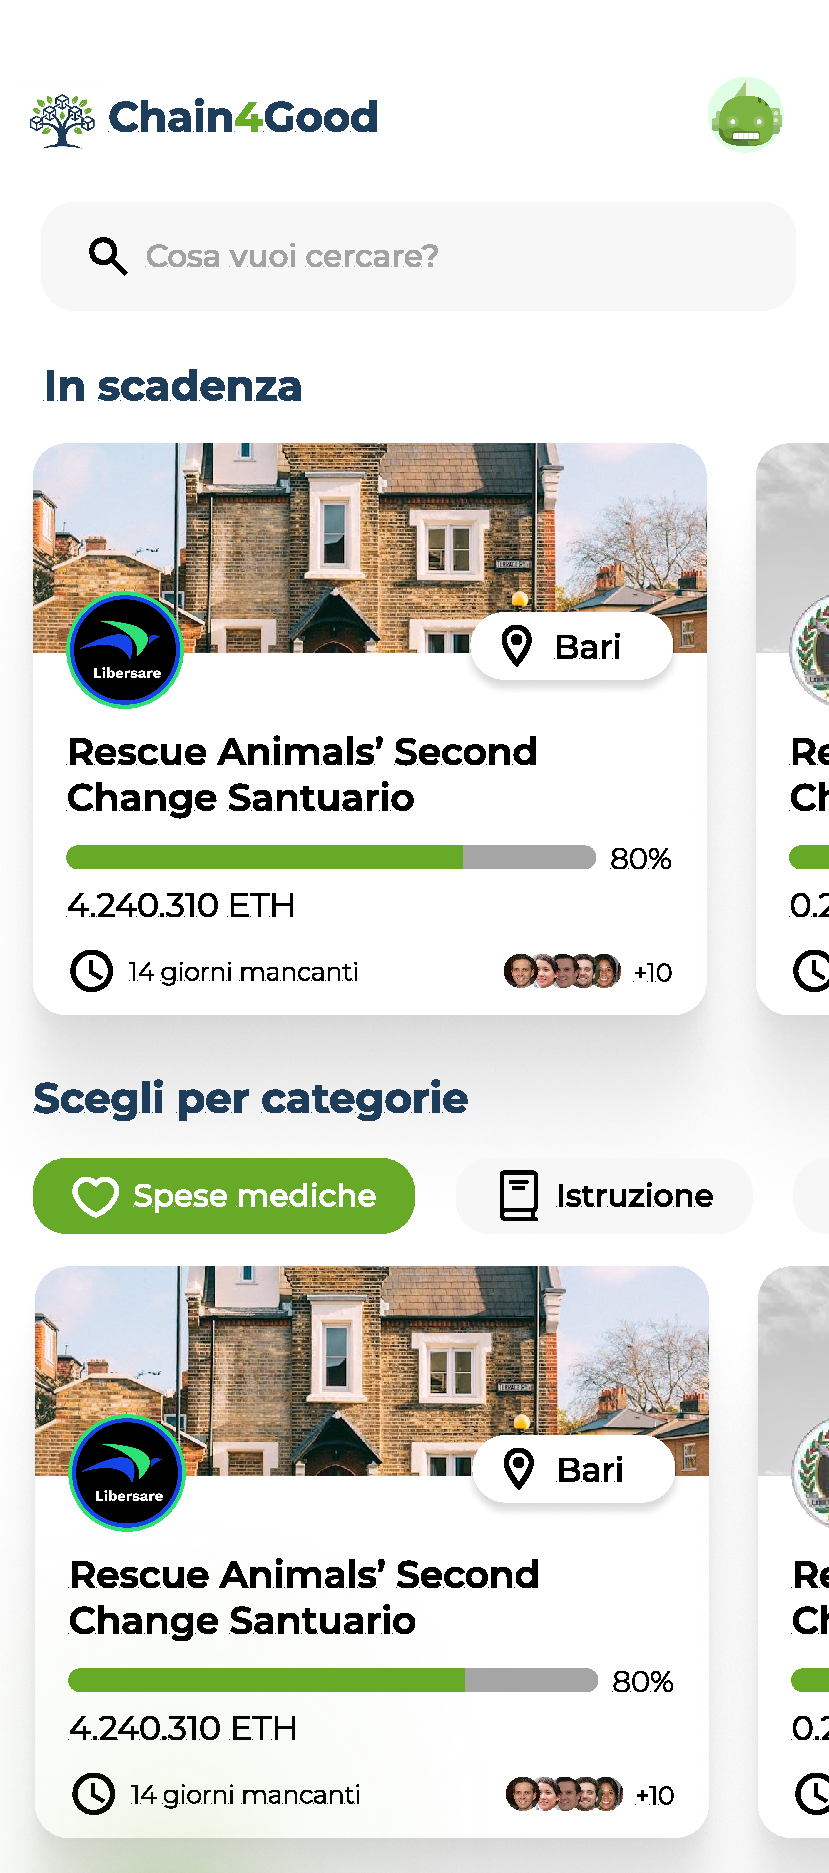
\includegraphics[width=0.40\textwidth]{images/Home_nuova.pdf}
	\caption{Dashboard del donatore}
	\label{fig:dashboard-donatore}
 \end{figure}
\clearpage


\subsection{Creazione progetto}
	La creazione di un progetto costituisce l’atto attraverso il quale il beneficiario formalizza la propria proposta sulla piattaforma. Tale procedura si articola in due step (\ref{fig:inserimento progetto}):

\begin{itemize}
	
	\item Step 1: l'Ente è tenuto a specificare le informazioni fondamentali del progetto, quali il nome, la categoria di appartenenza, l’obiettivo economico e il termine temporale della raccolta fondi. \\ 
	Gli ultimi due parametri permettono di automatizzare la gestione delle risorse in modalità \textit{trustless}, in quanto vengono utilizzati dallo \textit{Smart Contract} per determinare l’esito della raccolta fondi;
	
	\item Step 2: prevede l’inserimento di un piano dettagliato delle spese, oltre ad una descrizione approfondita del progetto e un’immagine di copertina. Tale prospetto non assolve solo finalità informative, ma contribuisce ad incrementare la credibilità dell'iniziativa e a consolidare il rapporto di fiducia con i donatori. 
	
\end{itemize}


\subsection{Inserimento e valutazione spesa}
A differenza dei sistemi centralizzati in cui l'Ente ha piena e immediata disponibilità del \textit{budget} donato, l’architettura proposta prevede che i fondi raccolti rimangano vincolati all'interno di uno \textit{Smart Contract}. \\
Per poter accedere a tali risorse, il beneficiario deve presentare una "Richiesta di Spesa" (\ref{fig:valutazione-spesa}) specificando il nome della spesa, l'importo richiesto, la finalità dell'esborso e il relativo preventivo. 
La sottomissione della richiesta è consentita esclusivamente quando il progetto si trova in uno stato attivo, ossia a seguito del raggiungimento del \textit{target} di raccolta oppure al termine della scadenza temporale prevista per la campagna. \\
A seguito della sottomissione, la richiesta viene poi sottoposta a un meccanismo di valutazione decentralizzato, basato sul voto dei donatori che hanno contribuito al finanziamento del progetto.
Coerentemente con la natura della piattaforma, il sistema di voto è stato implementato in modo da attribuire lo stesso peso a ciascun utente, indipendentemente dall'importo della donazione effettuata. Questa scelta progettuale è finalizzata a evitare che il potere decisionale risulti influenzato dalla capacità economica dei singoli utenti.\\
Al fine di assicurare un utilizzo progressivo e verificabile delle risorse raccolte, inoltre, la presentazione di una nuova richiesta di spesa è subordinata al caricamento della prova di acquisto relativa all’ultima richiesta precedentemente approvata. 
Tale approccio mira a garantire un utilizzo progressivo e verificabile dei fondi raccolti, e ad assicurare la conformità delle spese per le finalità dichiarate. 

\begin{figure}[t]
	\centering
	\begin{minipage}{0.37\textwidth}
		\centering
		\includegraphics[width=\textwidth]{images/nuovo_progetto1.pdf}
	\end{minipage}
	\hspace{1.5cm}
	\begin{minipage}{0.37\textwidth}
		\centering
		\includegraphics[width=\textwidth]{images/NuovoProgetto 2.pdf}
	\end{minipage}
	\caption{Inserimento di un nuovo progetto}
	\label{fig:inserimento progetto}
\end{figure}


\clearpage

\subsubsection{Meccanismo di votazione}
Per evitare lo stallo decisionale, lo \textit{Smart Contract} è stato programmato per gestire le richieste di spesa attraverso un periodo di votazione di durata prefissata pari a tre giorni, al termine del quale l’esito viene determinato secondo le seguenti regole:

\begin{itemize}
	\item \textbf{Approvazione per maggioranza alla scadenza}: la richiesta è approvata se, al termine del periodo di votazione, il numero di voti favorevoli è almeno pari ai voti contrari;
	
	\item \textbf{Approvazione anticipata per maggioranza matematica}: il sistema prevede la chiusura anticipata della votazione qualora il numero di pareri favorevoli raggiunga una soglia tale da rendere l'esito finale non più invertibile, anche nell'ipotesi in cui tutti i restanti aventi diritto esprimessero un voto contrario;
	
	\item \textbf{Parità dei voti}: qualora, allo scadere del periodo di votazione, si verifichi una situazione di parità tra voti favorevoli e contrari, la richiesta viene considerata approvata;

	\item \textbf{Mancata partecipazione}: nel caso in cui non venga espresso alcun voto entro la scadenza, il sistema approva automaticamente la richiesta al fine di non ostacolare l’avanzamento del progetto.
	
\end{itemize}

Al soddisfacimento di una delle condizioni di approvazione sopra elencate, lo \textit{Smart Contract} esegue in modo autonomo e irreversibile il trasferimento della somma richiesta verso il \textit{wallet} del beneficiario.

% funzione per donare - funzione per aggiungere la spesa - funzione per il voto



\begin{figure} [h]
	\centering
	\begin{minipage}{0.37\textwidth}
		\centering
		\includegraphics[width=\textwidth]{images/nuova_spesa.pdf}
	\end{minipage}
	\hspace{1.5cm}
	\begin{minipage}{0.37\textwidth}
		\centering
		\includegraphics[width=\textwidth]{images/valutazione_spesa.pdf}
	\end{minipage}
	\caption{Valutazione di una richiesta di spesa}
	\label{fig:valutazione-spesa}
\end{figure}




